Mit dem Weltraumteleskop Hubble wurde festgestellt, dass sich im Zentrum der Galaxie M84, in \dMeO\ Entfernung von uns, eine sehr grosse Masse befinden muss. Überprüfen Sie, ob im folgenden Zeitungsartikel die genannten Zahlen physikalisch zusammenpassen.

(Hinweis: Die Geschwindigkeiten sind die Bahngeschwindigkeiten von Objekten, welche um das Schwarze Loch kreisen.)

\begin{center}
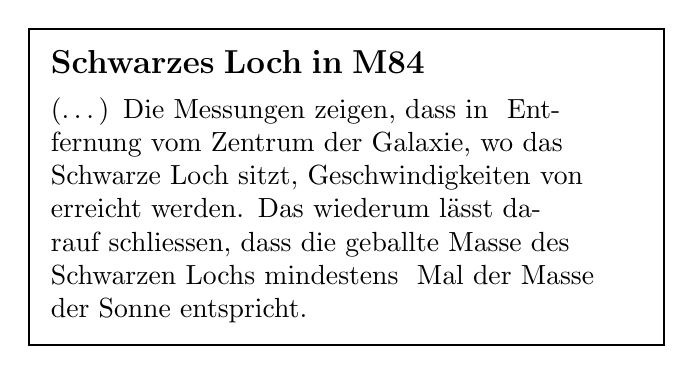
\begin{tikzpicture}
 \node[draw, thick, inner sep=8pt, text width=7.5cm, align=left] {\textbf{\large Schwarzes Loch in M84}\\[4pt]
 (\dots) Die Messungen zeigen, dass in \rLjO\ Entfernung vom Zentrum der Galaxie, wo das Schwarze Loch sitzt, Geschwindigkeiten von \vBO\ erreicht werden. Das wiederum lässt darauf schliessen, dass die geballte Masse des Schwarzen Lochs mindestens \nZO\ Mal der Masse der Sonne entspricht.};
\end{tikzpicture}
\end{center}
